% Monster stat block

   

\begin{figure*}[h!] % Example of a spanning figure
  \captionsetup[subfigure]{justification=centering}
    \centering
    \begin{subfigure}{0.4\textwidth}
        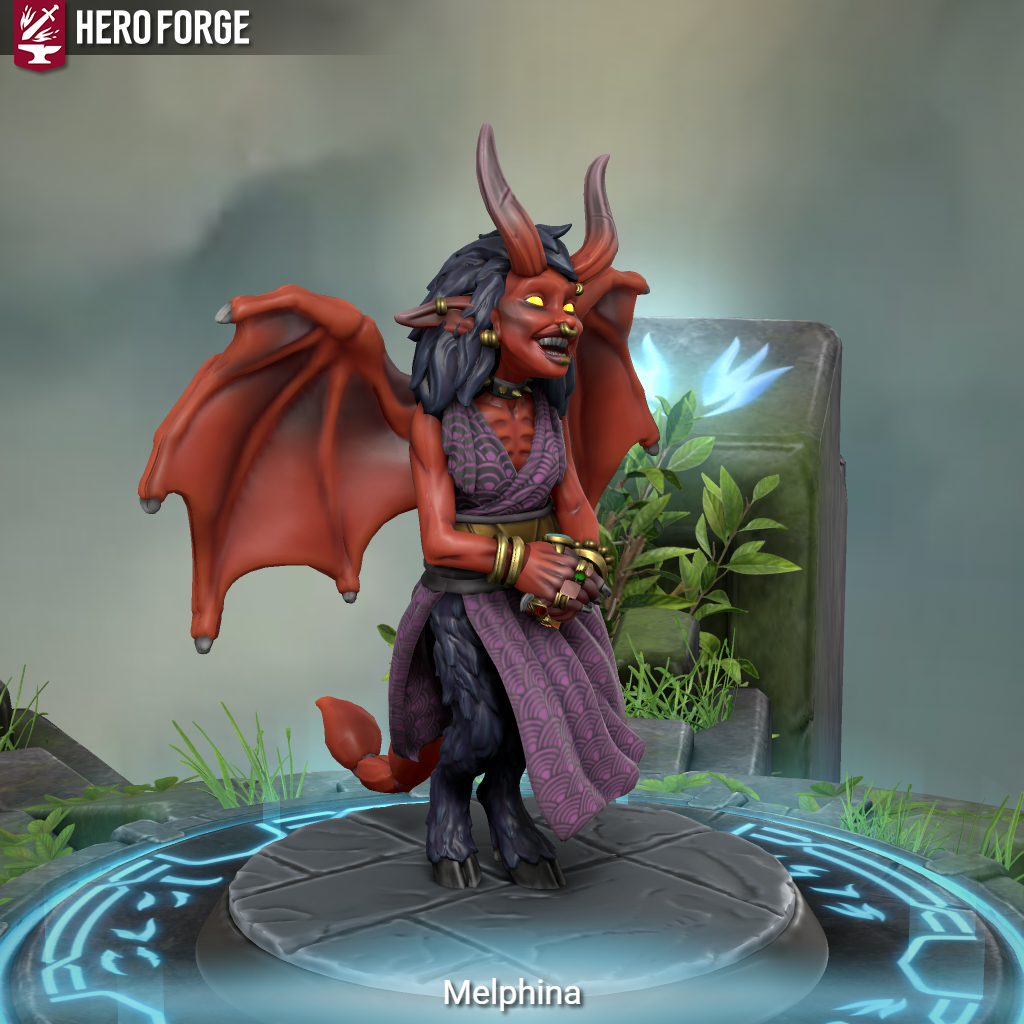
\includegraphics[width=\textwidth]{images/Thalvarien/Melphina_screenshot.png}
        \caption{Melphina}
    \end{subfigure}
    \hfill
    \begin{subfigure}{0.4\textwidth}
        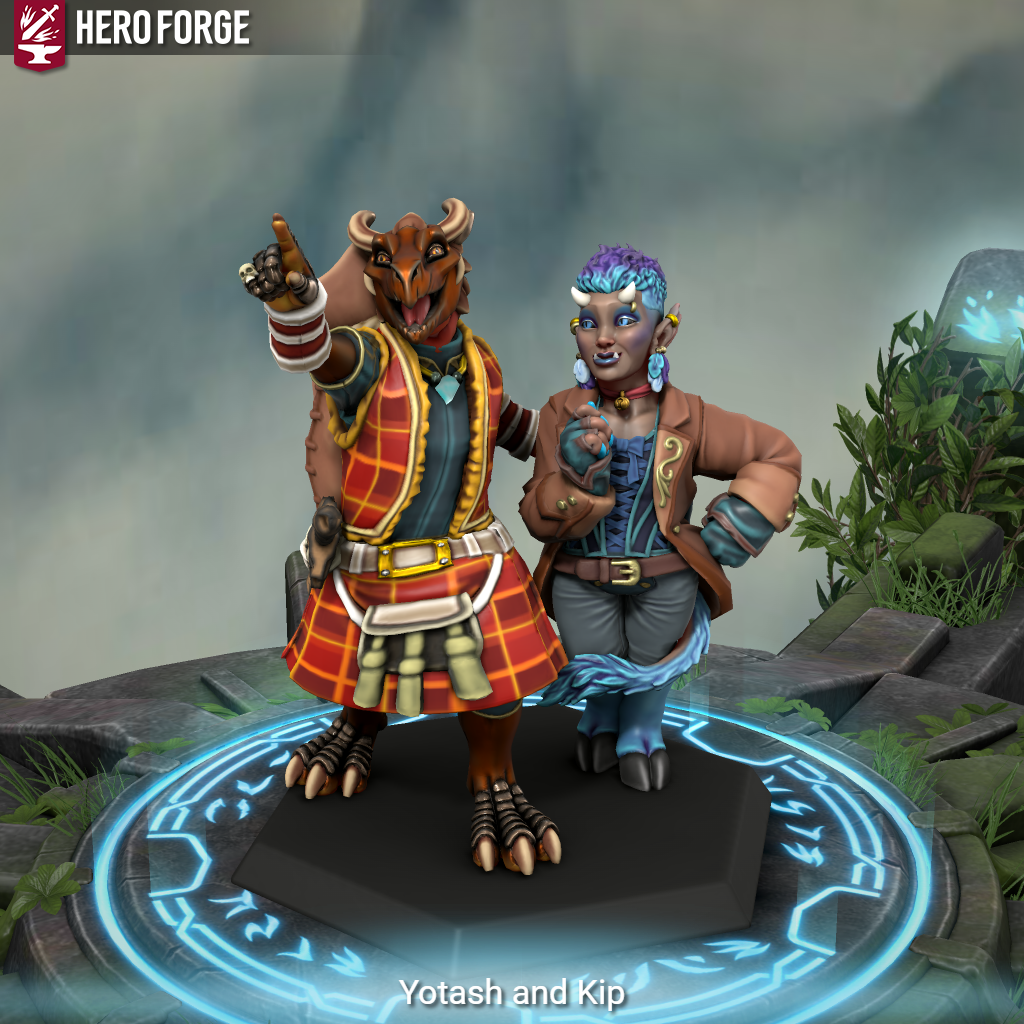
\includegraphics[width=\textwidth]{images/Thalvarien/Yotash_and_Kip_screenshot.png}
        \caption{Yotash \& Kip}
    \end{subfigure}
    \hfill
    \begin{subfigure}{0.4\textwidth}
        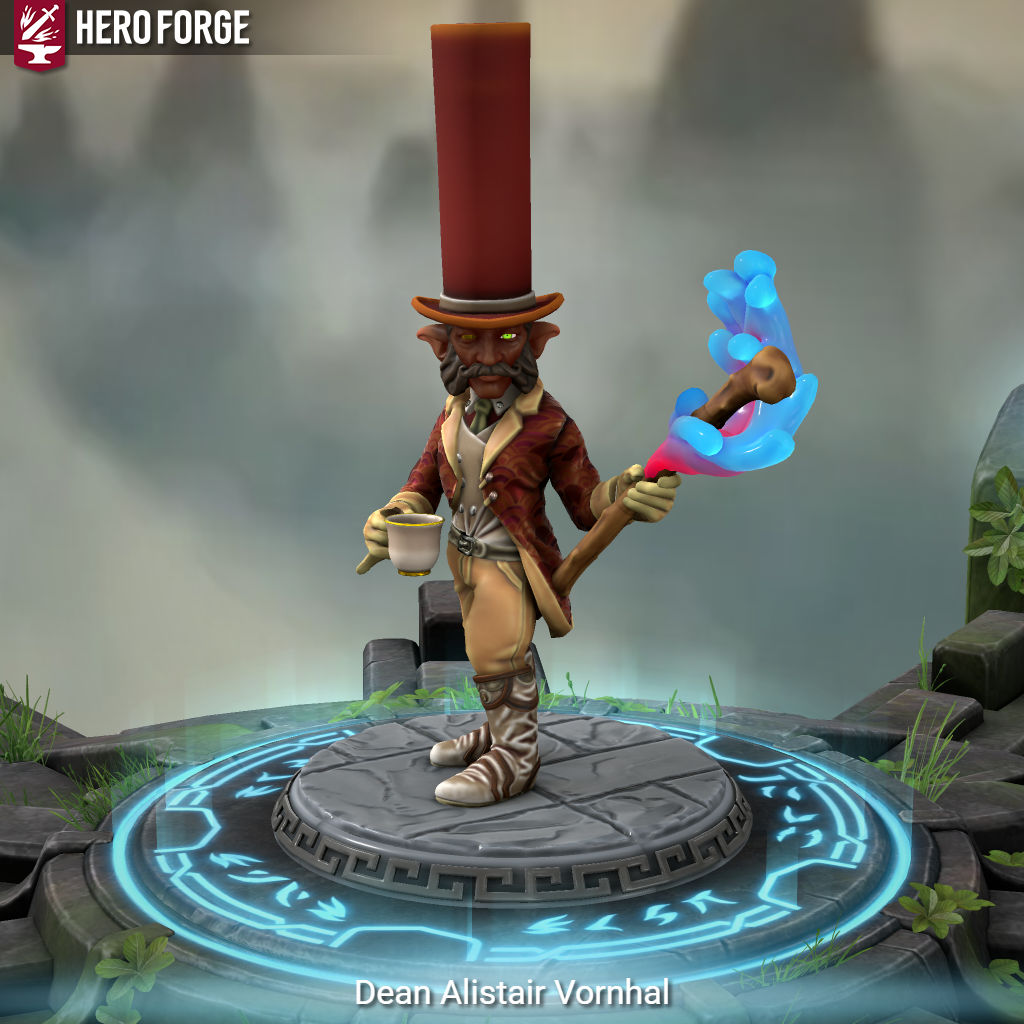
\includegraphics[width=\textwidth]{images/Thalvarien/Dean_Alistair_Vornhal_screenshot.png}
        \caption{Dean Alistair Vornhal}
    \end{subfigure}
    \hfill
    \begin{subfigure}{0.4\textwidth}
        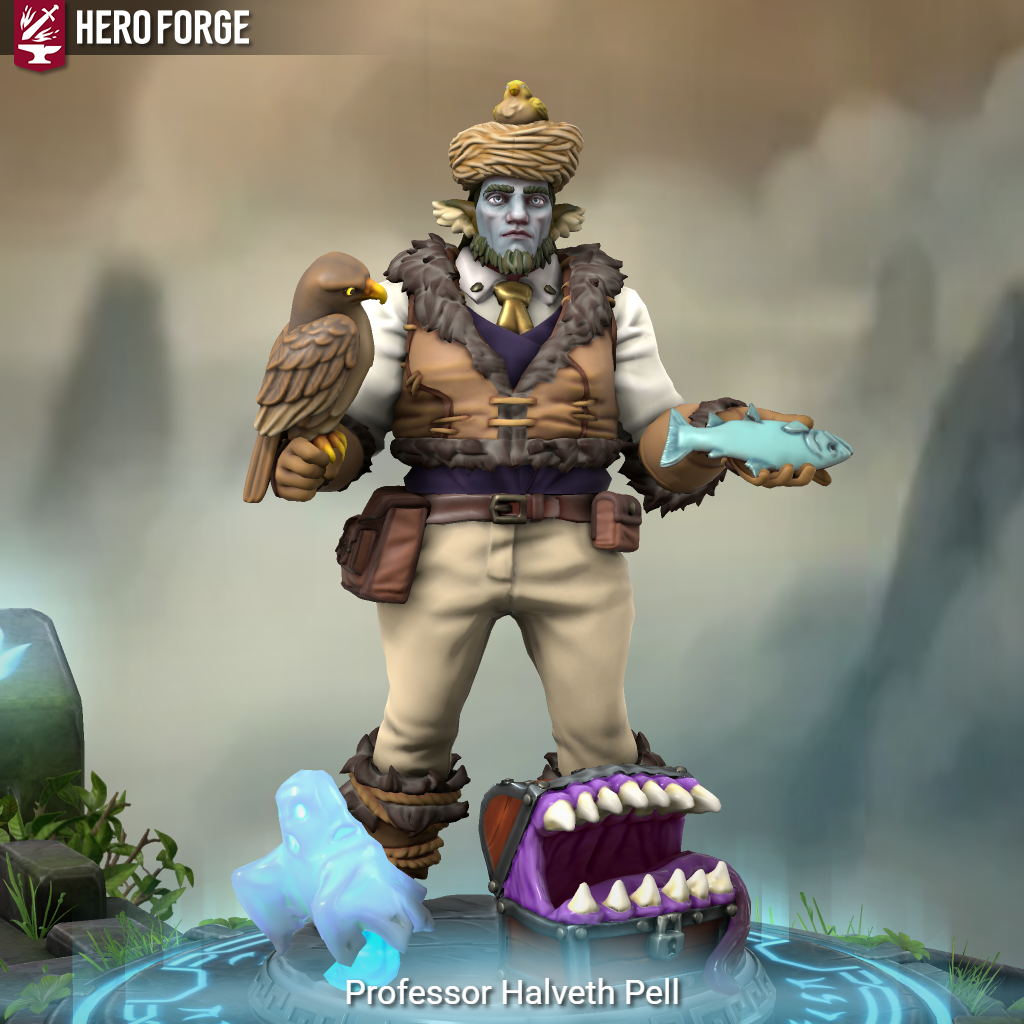
\includegraphics[width=\textwidth]{images/Thalvarien/Professor_Halveth_Pell_screenshot.png}
        \caption{Professor Halveth Pell}
    \end{subfigure}
    \hfill
    \begin{subfigure}{0.4\textwidth}
        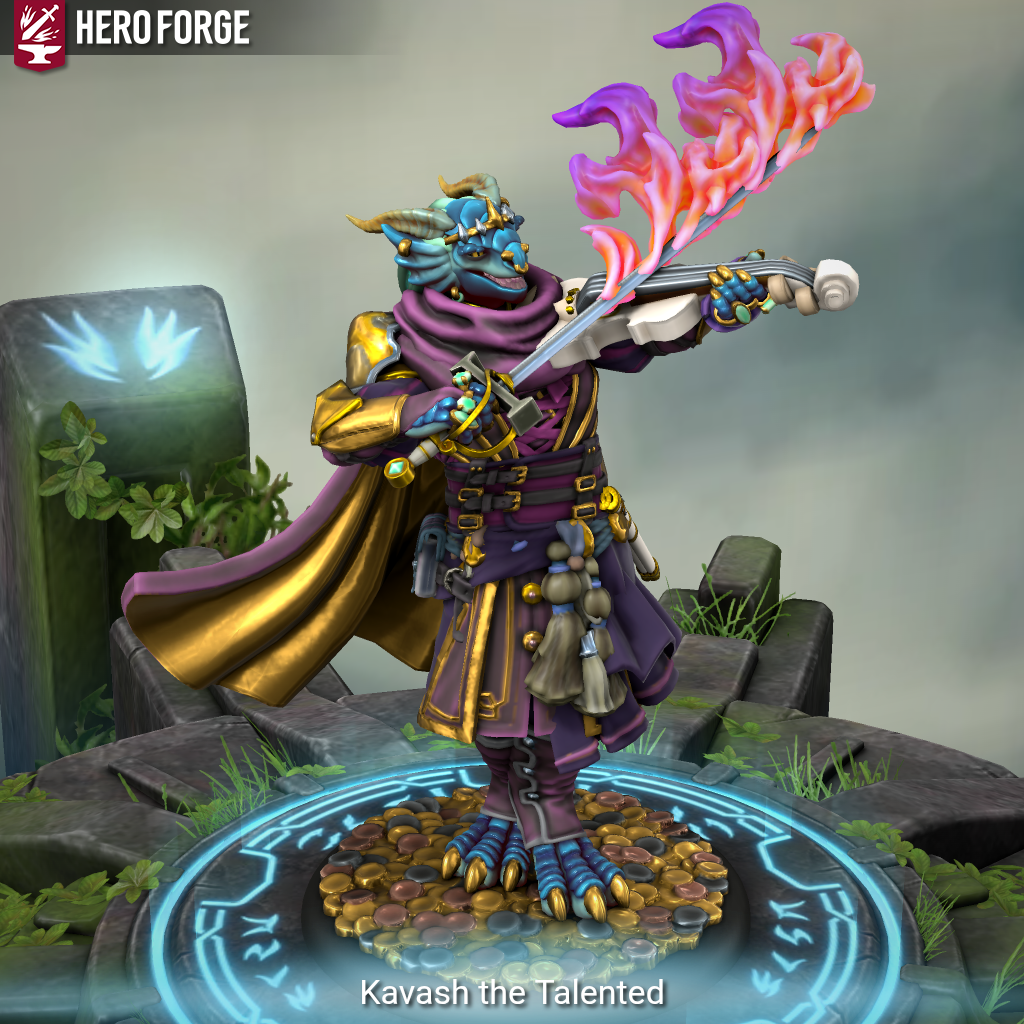
\includegraphics[width=\textwidth]{images/Thalvarien/Kavash_the_Talented_screenshot.png}
        \caption{Kavash The Talented}
    \end{subfigure}
    %\caption{Characters}
\end{figure*}


The |DndMonster| environment is used to typeset monster and NPC stat blocks. The module supplies many functions to easily typeset the contents of the stat block